\documentclass[dvipdfmx]{article}
\usepackage[dvipdfmx]{graphicx}
\usepackage{amsmath, amssymb}
\usepackage{mathtools}
\usepackage{here}
\begin{document}
\title{Weekly Report}
\author{Riku Gondow}
\maketitle
\section{Progress}
\begin{itemize}
    \item Continued to write bachelor thesis
    \item Did 10-fold cross validation under the close-set conditions and the open-set conditions on clean 30-subjects dataset
\end{itemize}

\section{10-fold cross validation}
10-fold cross validation was performed under the close-set conditions and the open-set conditions to confirm the classification accuracy. As shown in Fig.1, 2, we got 99.94\% (close-set) and 99.02\% (open-set).

\begin{table}[H]
\caption{Experimental parameters}
\centering
\begin{tabular}{cc}
\hline
Number of classes & 30 \\
Knowns classes (for open-set) & 15 \\
Unknowns classes (for open-set) & 15 \\
Batch size & 64 \\
Learning rate & 0.0001 \\
Window length (s) & 5 \\
Overlap (s) & 1.5 \\
Sampling rate (Hz) & 250 \\
\hline
\end{tabular}
\end{table}

\begin{figure}[H]
\begin{center}
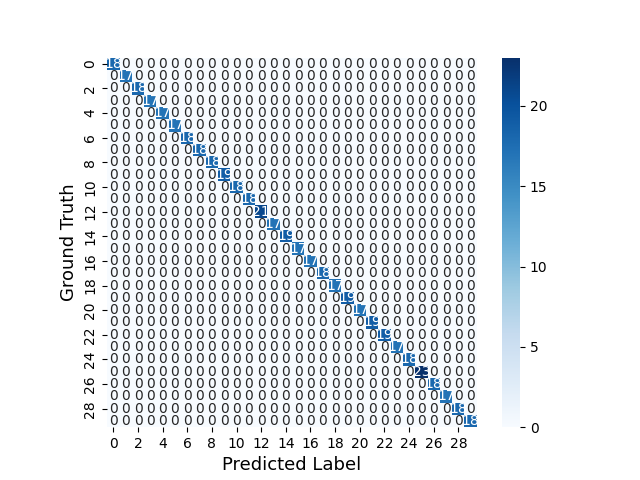
\includegraphics[width=0.8\linewidth]{./img/cross_val_Fold0_close.png}
\end{center}
\caption{Confusion matrix of 10-fold cross validation under the close-set conditions, Fold 0}
\end{figure}

\begin{figure}[H]
\begin{center}
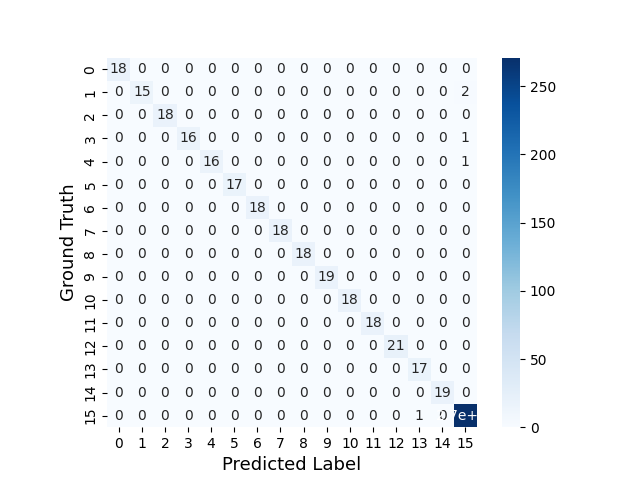
\includegraphics[width=0.8\linewidth]{./img/cross_val_Fold0_threshold0.8.png}
\end{center}
\caption{Confusion matrix of 10-fold cross validation under the open-set conditions, Fold 0, Threshold 0.8}
\end{figure}

\section{Next Plan}
\begin{itemize}
    \item Continue to write bachelor thesis
    \begin{itemize}
        \item Visualize feature maps
    \end{itemize}
    \item Perform 10-fold cross validation for Keio Hospital's Dataset
\end{itemize}

\end{document}